\section{基于Boosting的集成}
\label{sec:ensemble-boosting}

Bagging让多个成员分别完成同一个预测任务，再聚合它们的结果。如果这些成员反复在同一批样本上预测偏低，仅增加类似成员并平均，偏低的误差仍会保留。我们可以换一种训练方式：先计算已有组合还错在哪里，再让新成员专门学习一个修正量。

\term{Boosting}（提升）由此构造序贯加法模型：第$t$轮根据已有函数$F_{t-1}$选择新成员及其贡献，以降低指定训练目标。新成员承担的是对已有预测的补充，可以比一个独立完成任务的模型更简单。AdaBoost、梯度提升及现代提升树共享这种逐轮依赖，但它们从错误中提取修正信号的方式不同。

\subsection{前向逐步加法模型}
\label{sec:ensemble-stagewise-additive}

\subsubsection{模型结构}

设$F_0$为初始预测，Boosting经过$T$轮得到
\begin{equation}
  F_T(\bm{x})
  =
  F_0(\bm{x})
  +
  \sum_{t=1}^{T}\alpha_t h_t(\bm{x}),
  \label{eq:ensemble-additive-model}
\end{equation}
其中$h_t$是第$t$个成员，$\alpha_t$控制其贡献。

\subsubsection{参数学习}

为使复杂度惩罚对应真正加入模型的函数，把本轮增量记为$f_t=\alpha_t h_t$。给定损失$\ell$，理想化的第$t$轮直接优化增量：
\begin{equation}
  f_t
  \in
  \argmin_{f\in\mathcal{F}}
  \sum_{i=1}^{n}
  \ell\!\left(
    y_i,
    F_{t-1}(\bm{x}_i)+f(\bm{x}_i)
  \right)
  +\Omega_t(f).
  \label{eq:ensemble-forward-stagewise}
\end{equation}
这里$\mathcal{F}=\{\alpha h:\alpha\in\mathbb{R},h\in\mathcal{H}\}$是由成员函数族$\mathcal{H}$生成的增量函数族，$\Omega_t$是相应复杂度惩罚，也可以取零。

树的叶数惩罚控制分区规模，叶输出范数惩罚控制本轮增量。范数应作用于$f$，使惩罚随实际加入组合的幅度变化；若仅惩罚$h$，它与$\alpha$的相互缩放会改变惩罚却保持预测。

逐步优化固定已有成员，减少了联合搜索变量，但最优范围仅限本轮增量。后文用梯度拟合、二阶目标和收缩构造近似更新。

不同方法将当前预测转换为不同的训练信号。AdaBoost改变训练样本的权重，使当前错分记录在下一轮具有更大影响；梯度提升把损失对当前预测的负梯度作为伪响应；二阶提升树还利用局部曲率近似叶权重和分裂收益。平方损失的负梯度恰为普通响应残差，其他损失则给出不同修正量。损失决定了下一轮成员拟合的对象。

\subsection{AdaBoost}
\label{sec:ensemble-adaboost}

\subsubsection{模型结构}

先考虑二分类。如果每轮都用相同权重训练一个简单分类器，容易分类的多数样本可能反复决定边界，而少量错分样本始终得不到修正。\term{AdaBoost}（adaptive boosting）让错分记录在下一轮占更大权重，使新分类器更多地处理这些记录；同时根据本轮分类器的加权错误率确定它在组合中的贡献。这样，训练下一成员所面对的数据权重会随前面成员的预测改变。

模型以二分类函数作为成员，用加权得分$F_T(\bm{x})=\sum_{t=1}^T\alpha_t h_t(\bm{x})$表示组合，按其正负输出类别。每个成员只给出一个类别判断，投票权重决定该判断在组合中的作用。

\subsubsection{参数学习}

取标签$y_i\in\{-1,1\}$和成员$h_t(\bm{x})\in\{-1,1\}$。初始样本权重为$w_i^{(1)}=1/n$，第$t$轮成员的加权错误率为
\begin{equation}
  \epsilon_t
  =
  \sum_{i=1}^{n}
  w_i^{(t)}
  \mathbb{I}\!\left\{y_i\neq h_t(\bm{x}_i)\right\}.
  \label{eq:ensemble-adaboost-error}
\end{equation}
当$0<\epsilon_t<1/2$时，成员投票权重取
\begin{equation}
  \alpha_t
  =
  \frac{1}{2}
  \log\frac{1-\epsilon_t}{\epsilon_t},
  \qquad
  w_i^{(t+1)}
  =
  \frac{
    w_i^{(t)}
    \exp\!\left[-\alpha_t y_i h_t(\bm{x}_i)\right]
  }{Z_t},
  \label{eq:ensemble-adaboost-update}
\end{equation}
其中$Z_t$使新权重和为1。错分样本满足$y_i h_t(\bm{x}_i)=-1$，权重乘上$e^{\alpha_t}$；正确样本的权重乘上$e^{-\alpha_t}$。

若$\epsilon_t=0$，在这些正权重下当前成员已分对全部训练样本，便直接输出$h_t$并停止，避免将发散系数代入更新（参考\BookSectionRef{sec:boosting}{卷3《基础、理论与可信性》第5章“二分类学习的可学习性”第5.6节“集成学习”}）。其余情况下，最终分类器在预先固定平局规则后按$\operatorname{sign}(\sum_t\alpha_t h_t(\bm{x}))$决策。正的成员贡献要求当前加权错误率小于$1/2$；条件未满足时，可停止本轮、调整训练或采用相应变体。

图\ref{fig:ensemble-adaboost-weight-update}将分类错误与下一轮权重连接起来。当前分类结果先改变样本权重，再由归一化后的权重决定下一轮成员看到的训练分布；错分记录因而获得更大的后续影响。

\begin{figure*}[htbp]
  \centering
  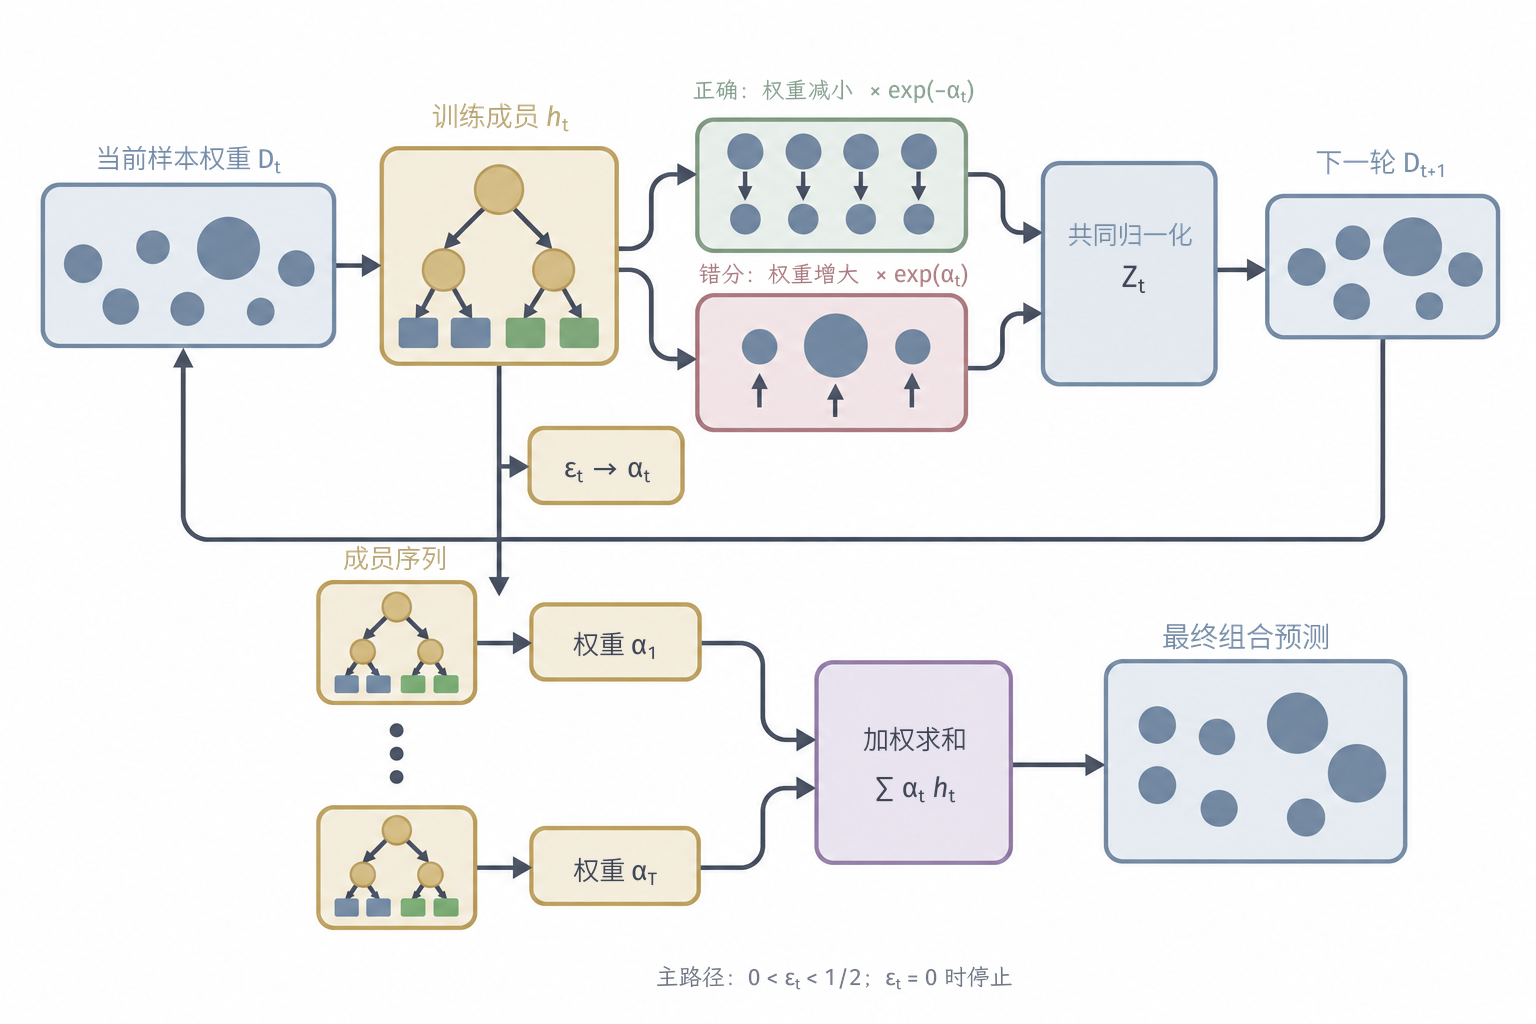
\includegraphics[width=130.048mm]{figures/04-classic-models/00-shared/generated/ensemble-adaboost-weight-update/figure.png}
  \caption{AdaBoost的样本权重更新。分类结果把样本分成正确与错分两路，两路缩放后的权重汇合并归一化，形成下一轮训练分布。实线连接各更新步骤；绿色框标示正确分类样本的减权，红色框标示错分样本的增权。}
  \label{fig:ensemble-adaboost-weight-update}
\end{figure*}

这一更新也可以从指数损失解释。令$F(\bm{x})=\sum_t\alpha_t h_t(\bm{x})$，经验目标为
\[
  \sum_{i=1}^{n}\exp\!\left[-y_iF(\bm{x}_i)\right].
\]
固定$F_{t-1}$后选择$h_t$与$\alpha_t$，在$0<\epsilon_t<1/2$时可以导出式\eqref{eq:ensemble-adaboost-update}。样本重加权由指数损失的逐步优化导出，因此其作用可以通过该目标分析\scite{freund1997boosting,friedman2000adaboost}。

\subsubsection{支持多分类预测场景}

二分类AdaBoost把每个成员的输出编码为$-1$或$+1$，最后用加权得分的正负判类。类别超过两个时，这个标量符号已经不能表示类别竞争。多分类变体需要让成员输出类别或逐类得分，再通过相应的加权投票或得分组合决定类别；样本重加权也要与所选多类损失一致。二分类中要求成员错误率低于$1/2$的条件及其系数公式不能直接沿用，必须按新的类别竞争方式重新推导。

\subsubsection{支持类别概率预测场景}

投票符号只回答类别，许多任务还需要输出事件发生的概率。LogitBoost从加法Logistic回归出发，用二项对数损失确定逐轮更新，再将累积得分转换为概率。它与AdaBoost都逐步加入成员，但修正量来自不同损失；转换后的概率是否准确，仍需根据样本外概率损失和校准情况判断\scite{friedman2000adaboost}。下一节给出一般损失如何导出修正信号的统一构造。

\subsection{梯度提升机与GBDT}
\label{sec:ensemble-gradient-boosting}

\subsubsection{模型结构}

AdaBoost用分类错误调整样本权重，但回归还需要描述“错了多少、向哪边修正”。例如，一个响应为100的样本当前预测为80，平方损失下需要向上修正；另一个响应同为100、当前预测为120的样本则需要向下修正。仅给两条记录增加相同权重，没有直接告诉新成员这两个相反方向。

对于关于预测可微的损失，负梯度给出了每个训练预测降低损失的方向。\term{梯度提升机}（gradient boosting machine, GBM）用基学习器拟合这些负梯度，再把学得的修正加入已有预测。取平方损失$\ell(y,F)=(y-F)^2/2$时，负梯度就是残差$y-F$，其他损失则产生各自的修正信号；序贯加法因而可以用于更一般的任务\scite{friedman2001gradientboost}。

GBM沿用式\eqref{eq:ensemble-additive-model}的加法结构，成员输出连续修正量。成员取回归树时，就是\term{梯度提升决策树}（gradient boosting decision tree, GBDT）；每片叶输出一个常数修正，全部树的修正叠加形成最终得分或数值预测。

\subsubsection{参数学习}

通常从使训练损失最小的常数预测开始：
\begin{equation}
  F_0(\bm{x})=c_0,
  \qquad
  c_0\in\argmin_c\sum_{i=1}^{n}\ell(y_i,c).
  \label{eq:ensemble-gbm-initialization}
\end{equation}
平方损失下$c_0$是响应均值。这里要求存在有限的最小化点；若某种损失与数据组合使最优常数趋于无穷，就需约束预测范围或另定有限初始化。

在第$t$轮，对每个训练样本计算\term{伪残差}（pseudo-residual），即损失在当前预测处的负导数：
\begin{equation}
  r_i^{(t)}
  =
  -
  \left.
  \frac{\partial \ell(y_i,z)}{\partial z}
  \right|_{z=F_{t-1}(\bm{x}_i)}.
  \label{eq:ensemble-pseudo-residual}
\end{equation}
随后用平方误差把这些修正量拟合到成员函数族：
\begin{equation}
  h_t\in\argmin_{h\in\mathcal{H}}
  \sum_{i=1}^{n}\bigl(r_i^{(t)}-h(\bm{x}_i)\bigr)^2.
  \label{eq:ensemble-gbm-gradient-fit}
\end{equation}
此处平方误差衡量成员对负梯度的逼近，即使原任务采用其他损失也使用这一拟合对象。贪心树生长通常给出子问题的近似解。

固定$h_t$后，可以按原损失做整体线搜索，在最小值存在时取
\begin{equation}
  \alpha_t\in\argmin_\alpha
  \sum_{i=1}^{n}
  \ell\!\left(y_i,F_{t-1}(\bm{x}_i)+\alpha h_t(\bm{x}_i)\right).
  \label{eq:ensemble-gbm-line-search}
\end{equation}
此处$\alpha_t$是整棵树或整个成员共享的一个标量。加入预先选择的收缩系数$\eta\in(0,1]$后，
\begin{equation}
  F_t(\bm{x})
  =
  F_{t-1}(\bm{x})
  +
  \eta\alpha_t h_t(\bm{x}).
  \label{eq:ensemble-gradient-boosting-update}
\end{equation}


当$\ell(y,z)=\tfrac12(y-z)^2$时，式\eqref{eq:ensemble-pseudo-residual}给出$y_i-F_{t-1}(\bm{x}_i)$，恰好是普通残差。图\ref{fig:ensemble-boosting-residuals}展示一次这样的更新：新成员拟合的是第二幅图中的残差，再把它的输出加回已有预测。左侧原本偏高的预测随负残差降低，右侧原本偏低的预测随正残差升高；这组数据的平均平方损失也随之下降。

\begin{figure*}[tbp]
  \centering
  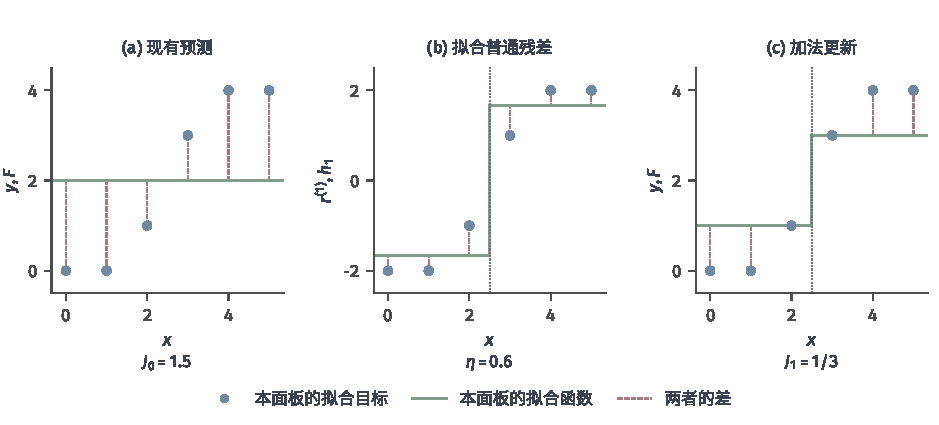
\includegraphics[width=159.000mm]{figures/04-classic-models/00-shared/matplotlib/ensemble-boosting-residuals/figure.pdf}
  \caption{平方损失下的一次梯度提升更新。六个输入为$x=0,\ldots,5$，响应依次为$0,0,1,3,4,4$，常数初始化$F_0=2$。在相邻输入中点中搜索，最小二乘残差树选取阈值$2.5$，两叶输出分别为$-5/3$与$5/3$。取$\eta=0.6$，$F_1=F_0+\eta h_1$在两侧分别为$1$与$3$；平均损失$J_t=(2n)^{-1}\sum_i[y_i-F_t(x_i)]^2$由$1.5$降至$1/3$。蓝点依次表示观测、残差、观测，绿线为各面板的拟合函数，红色虚线为两者之差。数据与更新均为可复核的教学构造，这个普通残差计算依赖平方损失。}
  \label{fig:ensemble-boosting-residuals}
\end{figure*}

分类时则要先明确得分与概率的关系。例如二分类采用$y_i\in\{0,1\}$，令$F$表示对数几率（logit），相应概率与二项对数损失为
\[
  p=\sigma(F)=\frac{1}{1+e^{-F}},\qquad
  \ell(y,F)=\log(1+e^F)-yF.
\]
由于$\partial\ell/\partial F=\sigma(F)-y$，第$t$轮的伪残差为
\[
  r_i^{(t)}=y_i-p_i^{(t-1)},\qquad
  p_i^{(t-1)}=\sigma\!\left(F_{t-1}(\bm{x}_i)\right).
\]


例如$y_i=1$而当前概率为$0.3$时，伪残差为$0.7$，表示损失对得分的修正信号。成员拟合后将增量加到$F$，再经Sigmoid换算概率；修正量与概率因此处于不同数值空间。

对于GBDT，除了整体线搜索，还可以保留平方拟合得到的叶区域$\bm{R}_1^{(t)},\ldots,\bm{R}_{L_t}^{(t)}$，再按原损失分别求每片叶的增量。当各叶内存在有限最小化点时，
\begin{equation}
  \begin{aligned}
    v_j^{(t)}
      &\in\argmin_v
        \sum_{i:\,\bm{x}_i\in\bm{R}_j^{(t)}}
        \ell\!\left(y_i,F_{t-1}(\bm{x}_i)+v\right),\\
    F_t(\bm{x})
      &=F_{t-1}(\bm{x})
        +\eta\sum_{j=1}^{L_t}
        v_j^{(t)}\mathbb{I}\{\bm{x}\in\bm{R}_j^{(t)}\}.
  \end{aligned}
  \label{eq:ensemble-gbm-leaf-update}
\end{equation}
$L_t$表示叶数，各叶分别选择$v_j^{(t)}$并替换原树输出；这与整棵树共用一个$\alpha_t$是两种更新方案。有限叶内最小值不存在时，需要限制输出或增加正则后再更新。回归树在这里承担连续修正量的拟合，最终任务也可以是分类。

\subsubsection{优化泛化能力}

\paragraph{控制逐轮更新幅度与模型复杂度}
学习率、轮数与单树复杂度共同决定加法函数。较小学习率缩小每轮变化，通常需要更多轮才能达到相近训练目标；较深的树可以在单轮表达更高阶交互，也会扩大每轮容量。行采样和列采样进一步引入随机性，早停则依据独立验证轨迹选择轮数。选择学习率时需同时调整轮数，并在给定树复杂度、采样和早停协议下比较。

\paragraph{减弱逐轮拟合对训练样本的依赖}
每轮都使用全部训练样本时，提升树可能反复追踪其中的偶然起伏。随机梯度提升在每轮只用一个随机子样本拟合新成员，使不同轮次面对的记录有所变化。它保留负梯度修正的目标，同时减少本轮参与拟合的样本数。子样本比例过低也可能使修正方向更不稳定，因此采样比例需要与学习率、轮数及树复杂度共同选择\scite{friedman2002stochastic}。

\paragraph{减弱新增成员对既有树的依赖}
提升的后期成员面对的是已有组合留下的残差，可能只修正少量记录，越来越依赖前面树的具体输出。DART在本轮计算修正信号时暂时移除一部分已有树，让新树补充这个不完整组合的预测。加入新树后，算法还会调整新树和被移除树的贡献，再将它们放回组合，避免补回同一缺口时使更新幅度过大。这里扰动的是已有预测，随机梯度提升扰动的则是本轮样本；两者可分别改变新成员依赖的信息，收益仍取决于扰动强度和任务\scite{rashmi2015dart}。

\subsubsection{支持分位数预测场景}

平方损失关注条件均值；若希望按允许的缺货概率确定库存阈值，或预测收入分布中的较低分位点，就需要条件分位数。把第\ref{sec:regression-quantiles}节的分位数损失$\ell(y,z)=\rho_\tau(y-z)$用于提升，成员便学习怎样减少这个分位数目标的偏差。由于损失在$z=y$处不可微，修正信号改用负次梯度，例如约定
\begin{equation}
  r_i^{(t)}
  =\tau-\mathbb{I}\{y_i<F_{t-1}(\bm{x}_i)\},
  \qquad 0<\tau<1.
  \label{eq:ensemble-quantile-pseudo-residual}
\end{equation}
等号处的负次梯度可取$[\tau-1,\tau]$内任意值，这里选端点$\tau$。常数初始化取样本$\tau$分位数，仍用平方误差拟合上述修正量；逐叶更新则最小化原分位数损失，故$v_j^{(t)}$取该叶内普通残差$y_i-F_{t-1}(\bm{x}_i)$的$\tau$分位数，而不是伪残差的均值。

\subsection{XGBoost}
\label{sec:ensemble-xgboost}

\subsubsection{模型结构}

前面介绍的梯度提升用负梯度决定修正方向。用树拟合时，还要选择怎样划分叶区域，以及每个叶应当输出多大的修正。只看当前梯度，没有直接利用损失随修正幅度弯曲的程度；若不断增加叶节点来追逐小幅训练收益，树也可能把样本噪声保留下来。

\term{XGBoost}把叶数和叶权重惩罚写入加法树目标，再用损失的二阶局部近似为叶输出和候选分裂评分。梯度描述向哪边修正，曲率参与决定修正幅度，正则项则限制这次修正使用多复杂的树。大规模训练还要处理稀疏特征、候选阈值与内存访问，原论文围绕这些计算设计了相应系统\scite{chen2016xgboost}。

\subsubsection{参数学习}

设第$t$棵树为$f_t$，损失在当前预测$F_{t-1}(\bm{x}_i)$处的一阶导与二阶导分别为$g_i^{(t)}$和$s_i^{(t)}$。去掉与$f_t$无关的常数后，本轮目标近似为
\begin{equation}
  \widetilde{\mathcal{L}}^{(t)}
  =
  \sum_{i=1}^{n}
  \left[
    g_i^{(t)}f_t(\bm{x}_i)
    +\frac{1}{2}s_i^{(t)}f_t^2(\bm{x}_i)
  \right]
  +\gamma L
  +\frac{\lambda}{2}\sum_{j=1}^{L}v_j^2,
  \label{eq:ensemble-xgboost-objective}
\end{equation}
其中$L$是叶数，$v_j$是第$j$片叶的输出，$\gamma$惩罚新增叶，$\lambda$约束叶权重。若$I_j$表示落入第$j$片叶的样本索引，记
\[
  G_j=\sum_{i\in I_j}g_i^{(t)},
  \qquad
  S_j=\sum_{i\in I_j}s_i^{(t)}.
\]
在$S_j+\lambda>0$时，固定树结构的最优叶权重为
\begin{equation}
  v_j^\star=-\frac{G_j}{S_j+\lambda}.
  \label{eq:ensemble-xgboost-leaf-weight}
\end{equation}
把一个父叶分成左右子叶时，相应近似目标下降量为
\begin{equation}
  \operatorname{Gain}
  =
  \frac{1}{2}
  \left[
    \frac{G_{\mathrm{L}}^2}{S_{\mathrm{L}}+\lambda}
    +
    \frac{G_{\mathrm{R}}^2}{S_{\mathrm{R}}+\lambda}
    -
    \frac{(G_{\mathrm{L}}+G_{\mathrm{R}})^2}
         {S_{\mathrm{L}}+S_{\mathrm{R}}+\lambda}
  \right]
  -\gamma.
  \label{eq:ensemble-xgboost-split-gain}
\end{equation}
式\eqref{eq:ensemble-xgboost-split-gain}把当前损失的梯度、曲率与树复杂度放在同一个分裂准则中。增益评价局部二阶目标在当前分裂下的变化；贪心生长只搜索逐步形成的结构。

图\ref{fig:ensemble-gradient-xgboost}把一阶梯度提升与XGBoost的二阶树评分放在同一计算链中。左图用负梯度定义拟合对象，右图从候选区域的梯度统计计算叶权重和分裂增益；二阶统计扩展了本轮目标的近似信息，但没有改变逐轮加法更新的外层结构。

\begin{figure*}[htbp]
  \centering
  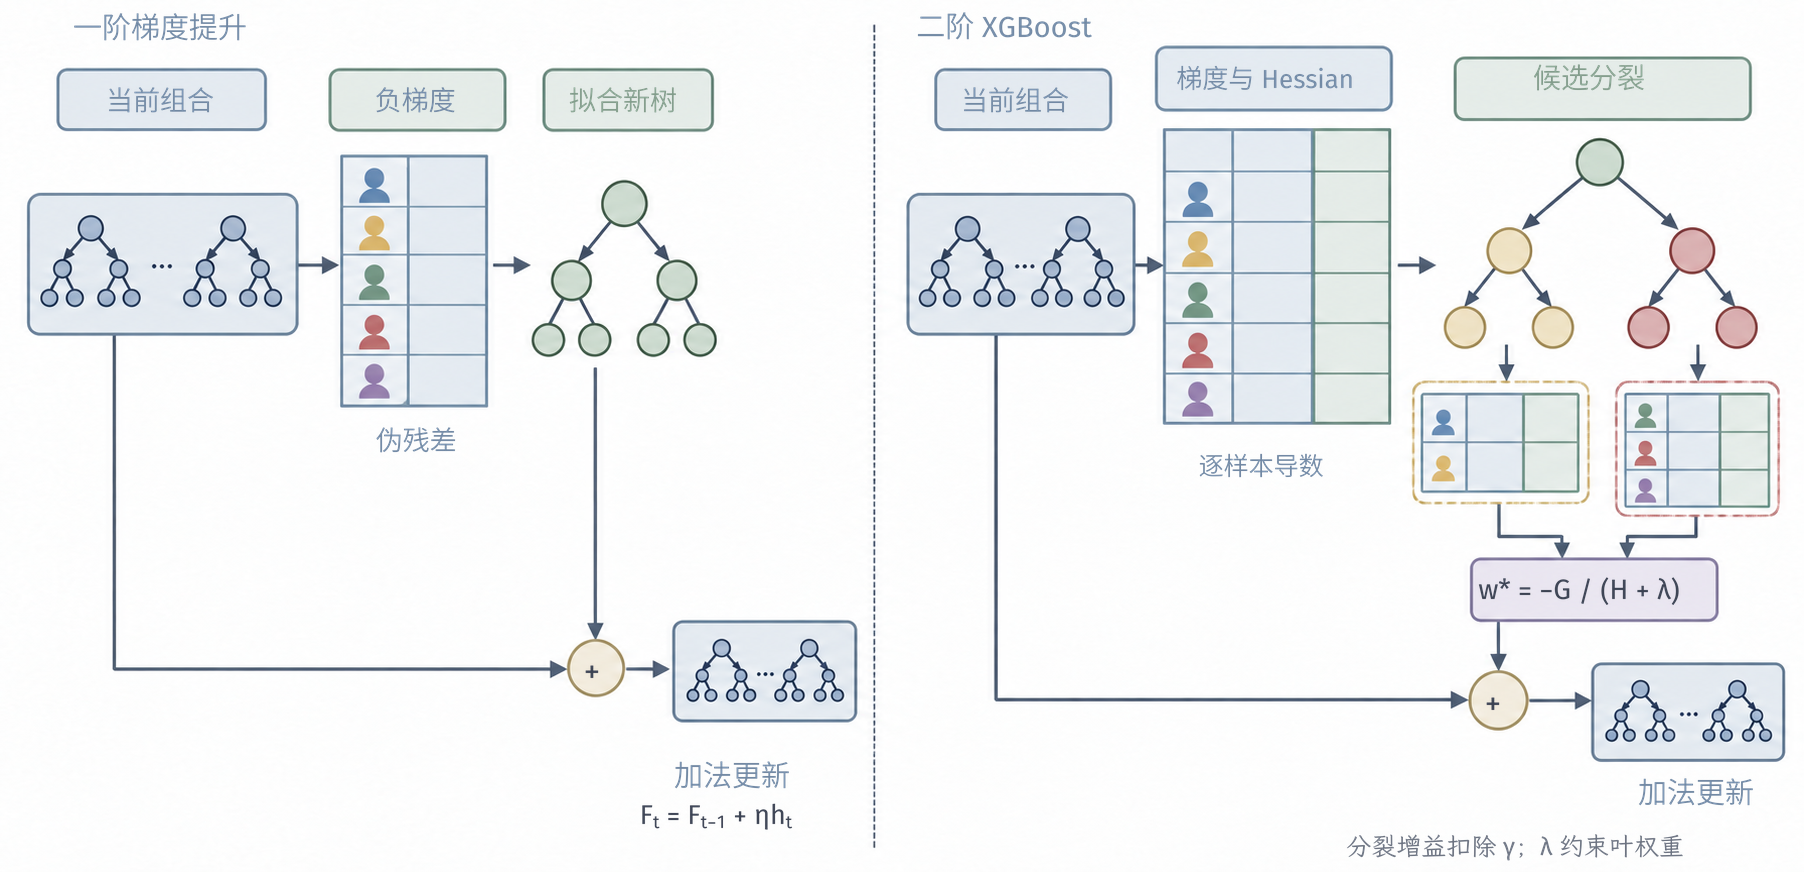
\includegraphics[width=152.739mm]{figures/04-classic-models/00-shared/generated/ensemble-gradient-xgboost/figure.png}
  \caption{梯度提升与XGBoost中的本轮修正。左图中，损失对当前预测的负梯度形成伪残差，新成员拟合该信号后更新组合；右图中，XGBoost按候选分裂聚合一阶导与二阶导，再由同一组叶统计计算叶权重和分裂增益。图中单叶权重$w^\ast$对应正文的$v_j^\star$，$G$与$H$分别表示叶内一阶导和二阶导之和。复杂度项$\gamma T+\lambda\lVert\bm{w}\rVert_2^2/2$中的$T$为叶数，$\bm{w}$汇集各叶输出；$\lambda$限制叶权重，$\gamma$惩罚新增叶。该图展示当前候选树的局部评分。}
  \label{fig:ensemble-gradient-xgboost}
\end{figure*}

\subsubsection{优化计算能力}

\paragraph{减少分裂搜索与数据访问}

精确分裂搜索遍历排序后的候选特征值；近似搜索则先用带权分位数草图构造候选切分，再汇总梯度统计。稀疏感知搜索为缺失值学习默认方向，列采样减少每轮需要检查的特征。块式存储、缓存感知访问、并行统计和外存计算改变的是实现代价，不改变式\eqref{eq:ensemble-xgboost-objective}所定义的学习对象。这些设计在特定硬件和数据规模上的时间收益可通过完整训练测量确认。

\Needspace{10\baselineskip}
\subsection{LightGBM}
\label{sec:ensemble-lightgbm}

\subsubsection{模型结构}

LightGBM仍以回归树的加法组合作为预测函数，树叶输出修正量，最终按任务所需把累计得分转换为预测。它主要改变如何在大规模数据上训练这些树。候选分裂的搜索可能成为提升树训练的主要成本。假设当前节点的一个连续特征有十万个不同取值，精确搜索就可能需要比较近十万个切分位置；每棵新树都会再次进行类似计算。\term{LightGBM}以直方图训练为基础，先把连续特征映射到有限个桶，再按桶累计梯度和曲率。如果使用256个桶，分裂评分就只在相邻桶之间比较，原来同桶内的差别被暂时忽略。

\subsubsection{参数学习}

构造直方图仍要访问节点样本，但候选搜索只需扫描桶。已知父节点和一个子节点的直方图时，还可以用差分得到另一个子节点的统计量。分桶减少存储和候选数，也引入离散化误差；桶数决定这种取舍。

树的生长顺序进一步改变计算分配。按层生长同时扩展某一深度上的叶，按叶生长则每次选择当前增益最大的叶继续分裂。在相同叶数下，后者把容量集中到训练目标下降较大的局部区域，可能形成深度不均衡的树。叶数、最小叶样本量和深度共同限制这种局部扩展，训练收益再由验证或测试检查其样本外效果。

\subsubsection{优化计算能力}

\paragraph{减少样本统计量}

基本直方图训练仍需统计大量样本和特征。LightGBM论文进一步提出两种针对这些成本的近似。\term{单边梯度采样}（gradient-based one-side sampling, GOSS）保留绝对梯度较大的样本，从绝对梯度较小的样本中随机抽取一部分，并在分裂统计中重新加权后者。例如，在小梯度组内等概率抽取一半样本，就把被抽中者对梯度和的贡献乘二，以补偿未采样部分。一般地，样本以概率$p>0$被保留时，其贡献乘以$1/p$；给定本轮梯度和候选分区，这种逆包含概率加权可无偏估计相应的梯度和，平方、比值及择优得到的增益则是非线性量，其偏差需另行分析。

\paragraph{减少有效特征数}

\term{互斥特征捆绑}（exclusive feature bundling, EFB）把很少同时非零的稀疏特征编码到较少的组合特征中，近似减少有效特征数。GOSS、EFB和直方图分别减少样本统计、特征表示和阈值候选，可按各自近似对象评价误差与计算节省\scite{ke2017lightgbm}。

图\ref{fig:ensemble-lightgbm-approximations}按近似对象并列这三种机制。直方图压缩候选阈值，GOSS压缩参与分裂统计的样本，EFB压缩稀疏特征表示；这三个对象分别对应数据访问、有效特征数与候选扫描的成本。

\begin{figure*}[t]
  \centering
  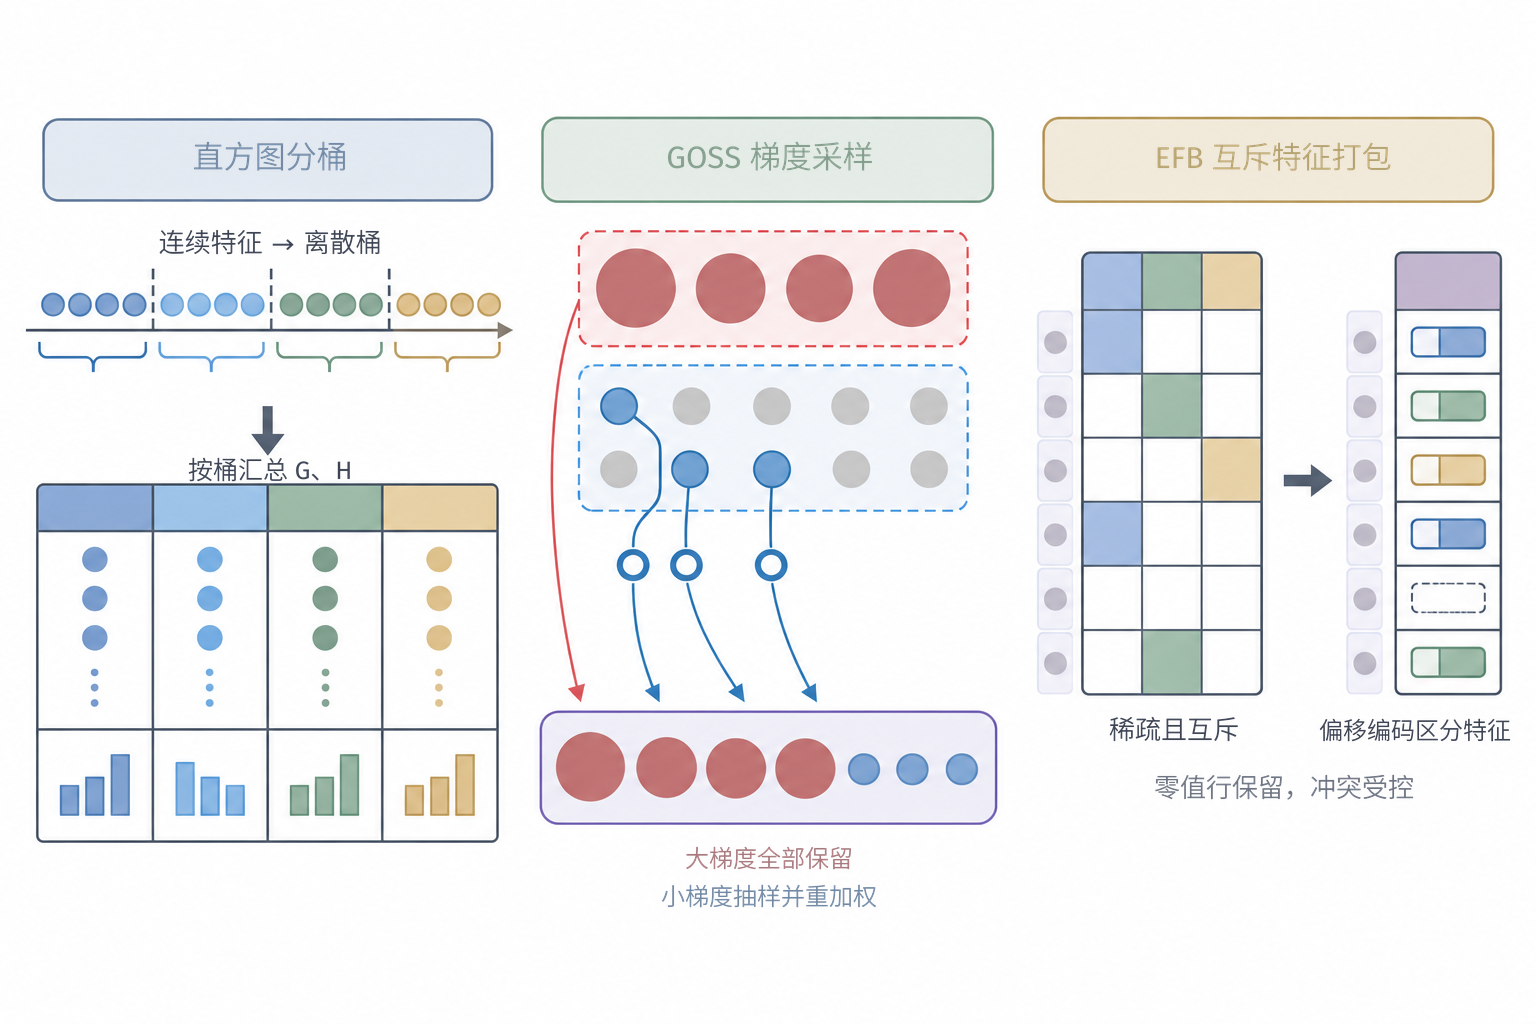
\includegraphics[width=130.048mm]{figures/04-classic-models/00-shared/generated/ensemble-lightgbm-approximations/figure.png}
  \caption{LightGBM中三种作用位置不同的计算近似。直方图把连续取值映射到有限桶，GOSS保留$|g_i|$较大的样本，并抽取、重加权部分$|g_i|$较小的样本，EFB把很少同时非零的特征编码为较少的捆绑特征。图中点数、桶数与非零位置均为机制示意。}
  \label{fig:ensemble-lightgbm-approximations}
\end{figure*}

这些机制的效果依赖梯度分布、特征稀疏性、桶数、冲突处理和硬件实现。比较速度和任务损失时，需要记录数据规模、硬件、桶数与采样设置，并固定搜索预算及早停规则。论文实验的结论据此限定于相应条件。GOSS对固定候选分区的梯度统计可以无偏，并不意味着据此选出的模型已经获得较低的期望风险。

\subsection{CatBoost}
\label{sec:ensemble-catboost}

\subsubsection{模型结构}

类别特征又带来不同的困难。例如商户标识可能有很多取值，全部展开为独热变量会增加特征规模，直接编成整数又会引入原本不存在的次序。用同类别记录的响应均值编码，可以把类别转成一个数，却容易把标签带回输入：某个商户若只有一条记录，包含该记录自身的响应均值恰好就是$y_i$，训练模型于是能直接读到待预测值。新记录的标签还未知，部署时无法提供同样信息。这种把待预测响应用于训练输入的构造称为\term{目标泄漏}（target leakage）。

\term{CatBoost}仍通过逐轮相加的树模型形成预测，并为类别特征安排避免当前标签泄漏的编码过程。它常使用\term{对称树}（symmetric tree），即同一深度的所有节点采用相同分裂条件。深度为$d_{\mathrm{tree}}$的完整对称树至多有$2^{d_{\mathrm{tree}}}$片叶，路径可以编码为固定长度的二进制选择。这种结构便于批量预测，也限制了单棵树可表达的分区形状。

\subsubsection{参数学习}

CatBoost用随机排列建立\term{有序目标统计}（ordered target statistic）。设$c_i$为样本$i$的某个类别值，用$\pi(j)$表示样本$j$在随机排列中的位置；对当前样本只使用排列中位于它之前且类别相同的记录：
\begin{equation}
  z_i
  =
  \frac{
    \sum_{j:\,\pi(j)<\pi(i)}
    \mathbb{I}\{c_j=c_i\}y_j
    +ap
  }{
    \sum_{j:\,\pi(j)<\pi(i)}
    \mathbb{I}\{c_j=c_i\}
    +a
  }.
  \label{eq:ensemble-catboost-ordered-statistic}
\end{equation}
其中$p$是先验统计量，$a>0$控制平滑。前缀统计排除了样本自身的标签，部署时可从已观测的训练记录形成同类别统计。低频类别仍会产生较大估计波动，平滑、多个排列和类别组合需要共同考虑。

图\ref{fig:ensemble-catboost-ordered-statistics}固定当前样本的排列位置，检查哪些标签进入编码。计算当前类别$A$样本的编码时，只允许排列前缀中同为类别$A$的标签进入统计量；其他类别、当前标签和排列后缀都不参与这次编码。

\begin{figure*}[htbp]
  \centering
  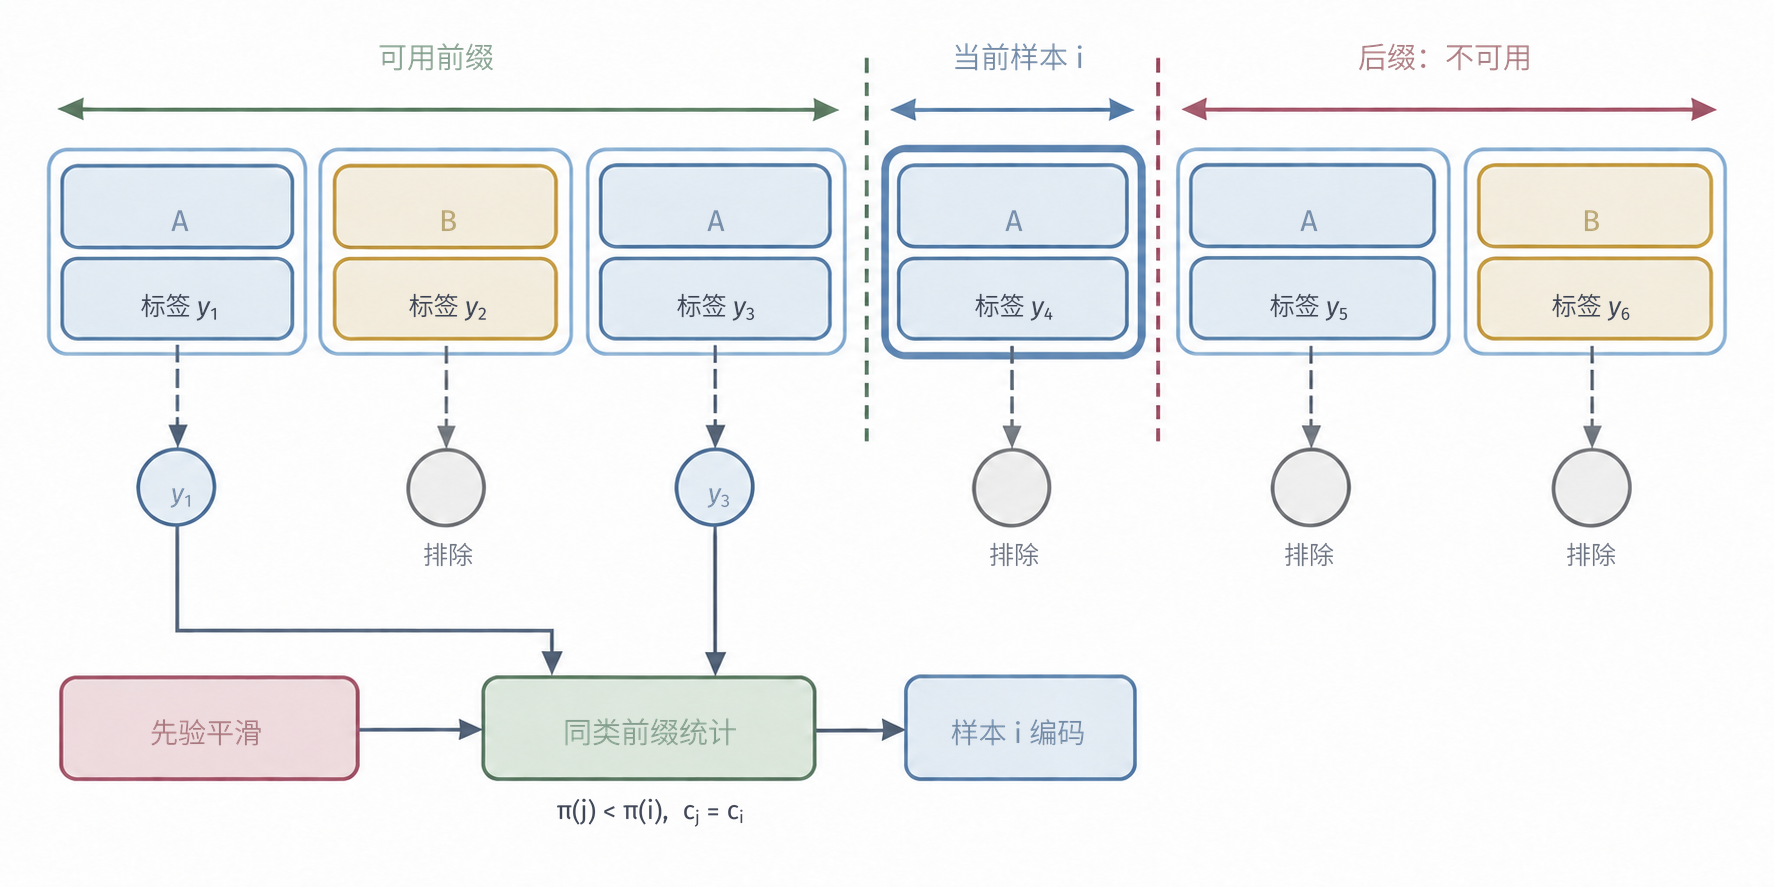
\includegraphics[width=150.199mm]{figures/04-classic-models/00-shared/generated/ensemble-catboost-ordered-statistics/figure.png}
  \caption{CatBoost有序目标统计的前缀约束。这里$\pi(j)$表示样本$j$在随机排列中的位置；计算当前样本$i$的编码时，只有满足$\pi(j)<\pi(i)$且$c_j=c_i$的标签通过实线汇入统计量。其他类别、当前标签和后续记录均不连接到统计量，表示它们在本次编码中被隔离。样本索引与类别符号仅用于说明机制。}
  \label{fig:ensemble-catboost-ordered-statistics}
\end{figure*}

有序提升把相同的前缀思想用于梯度估计。计算当前样本的预测与梯度时，采用由其前缀记录拟合的相应模型，使该样本的标签与当前预测拟合分离，以减少这一重复使用带来的预测偏移。实际算法通过多个排列和前缀模型实现这一约束，训练状态与计算量也比普通单序列提升更复杂\scite{prokhorenkova2018catboost}。

\subsection{模型对比与总结}
\label{sec:ensemble-boosting-comparison}

这些方法首先区别在“下一轮学什么”。AdaBoost由指数损失导出样本重加权，使错分记录影响后续分类器；GBM从一般损失导出负梯度，让成员拟合连续修正量，因而可以通过改变损失支持回归、概率分类和分位数预测。GBDT是以回归树拟合修正量的GBM实例。随机梯度提升和DART在这条序贯链上引入不同扰动，分别改变本轮样本与本轮所见的已有组合。

树提升还需要决定“怎样把修正量分配给叶区域”。XGBoost把损失曲率、叶权重惩罚和叶数代价合入局部评分，使候选分裂和叶输出可以用同一组统计计算。LightGBM进一步针对样本多、特征多、阈值候选多的计算成本，采用直方图、GOSS和EFB压缩相应对象，并按叶生长分配树容量。这些计算设计可以与损失及正则选择配合，代价是分桶、采样和特征捆绑带来的近似，不能仅凭方法名称判断速度或预测优劣。

CatBoost关注类别特征和标签重复使用的问题。它用排列前缀构造目标统计，并用前缀模型形成有序梯度，减少当前标签同时参与编码或预测拟合所造成的偏移；对称树则约束分区结构并便于批量预测。它与XGBoost、LightGBM共享树提升的外层结构，主要设计重点分别落在不同位置。表\ref{tab:ensemble-boosting-comparison}据此比较修正信号、局部目标、分裂计算与类别信息的使用方式。

\begin{table*}[htbp]
  \centering
  \small
  \begin{tabularx}{\linewidth}{@{}>{\raggedright\arraybackslash}p{19mm}*{6}{>{\raggedright\arraybackslash}X}@{}}
    \toprule
    方法 & 本轮修正信号 & 典型成员 & 目标近似 & 树生长或分裂 & 类别特征重点 & 主要约束 \\
    \midrule
    AdaBoost & 加权错分 & 树桩或浅分类树 & 指数损失下的解析更新 & 由成员算法决定 & 需另行编码 & 对持续错分记录敏感 \\
    GBM／GBDT & 负梯度伪残差 & 回归树 & 一阶函数方向与叶内优化 & 通常贪心树生长 & 需随实现处理 & 学习率、轮数与树复杂度耦合 \\
    XGBoost & 一阶导与二阶导 & 正则化回归树 & 二阶局部目标 & 精确或分位数候选；稀疏默认方向 & 依实现与版本而定 & 轮次串行，近似与系统配置影响成本 \\
    LightGBM & 桶级梯度统计 & 直方图回归树 & 通常使用二阶统计 & 按叶生长；直方图候选 & 支持类别分组，机制依实现 & 分桶、GOSS与EFB引入近似条件 \\
    CatBoost & 有序统计与有序梯度 & 对称树 & 梯度或二阶统计 & 同层共享分裂条件 & 有序目标统计与组合 & 多排列和前缀状态增加训练成本 \\
    \bottomrule
  \end{tabularx}
  \caption{Boosting代表方法的机制比较。GBM是一般框架，GBDT指使用回归树成员的实例；XGBoost、LightGBM和CatBoost是树提升的具体模型与系统，均属于Boosting框架的具体构造。}
  \label{tab:ensemble-boosting-comparison}
\end{table*}

提升方法都围绕当前组合继续训练，学习率、轮数和单树容量因而需要联合选择。若已有成员来自不同模型族，希望根据它们的样本外表现学习组合方式，就转向Stacking。
